\subsection{Analog-to-Digital Converter}

For at teste, hvorvidt ADC'en kan sample tre inputs, opsættes tre inputkanaler. 
Dette fremgår af \autoref{fig:treinput}.

\begin{figure}[H]
\centering
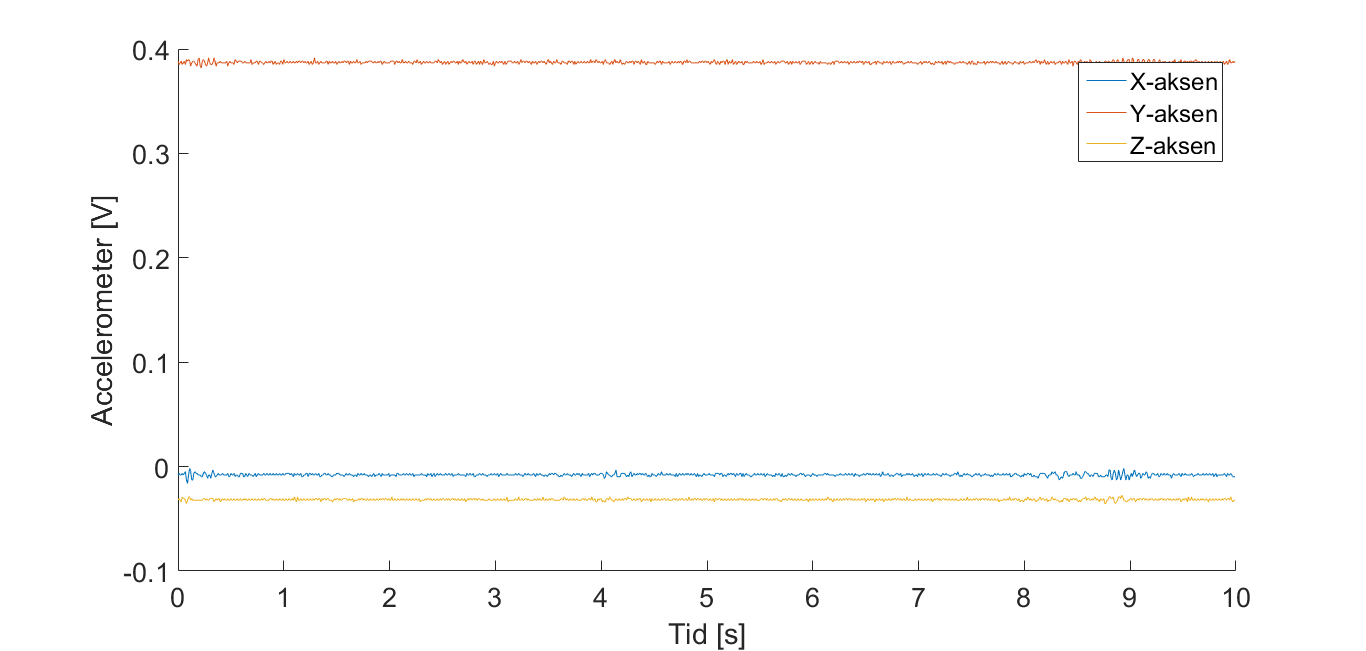
\includegraphics[width=1\textwidth]{figures/treinput}
\caption{Tre signaler samplet samt visualiseret i MATLAB. Signalerne er samplet fra et accelerometers tre akser under bevægelse af accelerometret.}
\label{fig:treinput}
\end{figure}

\noindent
Det ses på \autoref{fig:treinput}, at ADC'en kan sample tre signaler. 
Ligeledes ses det af figuren, at der ikke fremkommer tydelige LSB-trin, hvortil en opløsning på 11 bit antages som acceptabel.

%På baggrund af \autoref{sec:ADC_imp} er der valgt at anvende en ADC med et arbejdsområde på $2^{11}$, hvilket vurderes at være acceptabel og ikke forringer det ønskede signal under konverteringen. Dette ses ligeledes af \autoref{fig:treinput}.
Derudover fremgår det af \autoref{fig:treinput}, at signalet ikke overstiger ADC'ens arbejdsområde under store udsving af accelerometersignalet. 
Hertil forventes det, at signalet ikke overstiger arbejdsområdet ved det samlede system, da en lignende bevægelse fremkommer usandsynlig. 

Det blev påvist i \autoref{sec:pilotforsoeg}, at frekvensområdet for muskelaktiviteten efter, at det har passeret EMG-forstærkeren, befinder sig relativt lavfrekvent, mellem $0,4-10~Hz$. 
Hertil er en samplingsfrekvens på $100~Hz$  tilstrækkelig ud fra Nyquists sætning, som beskrevet i \autoref{sec:ADC_teori}.

%Det fremgår \autoref{sec:pilotforsoeg} at frekvensområdet for muskelaktivitet befinder sig relativt lavfrekvent mellem $0,4-10~Hz$. Derved anses en samplingfrekvens på $100~Hz$ tilstrækkeligt. 

ADC'ens samplingsfrekvens testes for at undersøge, om den indstillede og reelle samplerate er identisk. 
Til denne test defineres en variabel, som tæller op for hver gang, at der er konverteret data fra ADC'en. 
Hvis en konvertering mislykkes, vil den givne sample ikke registreres. 
De registrerede værdier videresendes via USB-forbindelse mellem computer og mikrokontroller, hvorefter dataen aflæses i MATLAB. 
Testen foretages i 30 minutter, hvor konvertering samt tid startes samtidigt. 
De registrerede data aflæses, hvorved en samplingsfrekvens udregnes i \autoref{eq:ADC_test}. 
Antallet af konverteringer målt under testen er $177.066~samples$ over en periode af $1.800,16~s$.

\begin{equation}\label{eq:ADC_test}
Fs = \frac{177.066~samples}{1.800,16~s}
\end{equation}

\noindent
Der forventes en samplingsfrekvens på $100~Hz$. 
Den reelle frekvens er udregnet til $98,36~Hz$ ud fra \autoref{eq:ADC_test}. 
Dette giver en afvigelse på $1,64\%$. 
Afvigelsen kan skyldes, at det ikke har været muligt at starte og stoppe tiden samt konverteringen på præcist samme tidspunkt. 
Dette betyder, at der ikke er en direkte relation mellem konverteringen og tiden. 

Der blev yderligere foretaget en test af samplingsfrekvensen ved brug af et oscilloskop. 
Dette gav en samplingsfrekvens på $98,43~Hz$, hvilket afviger fra den valgte samplingsfrekvens med $1,57\%$. 

De to afvigelser kan yderligere være forårsaget  af den samlede konverteringstid for de tre kanaler, der af \autoref{sec:ADC_bilag} er udregnet til $9,96~ms$. 
Dette opgiver ADC'en som en samplingsfrekvens på $100~Hz$, dog vil den reelle konverteringstid for de tre kanaler være $10~ms$.  
%fremgår det at Yderligere tillader indstillingerne for ADC'en, at der kan ændres i konverteringstiden for de enkelte kanaler, men samtidig oplyse, at der bevares en aktuel samplingsfrekvens på $100~Hz$. Dette antages ligeledes at have en indflydelse på samplingsfrekvensen, selvom den oplyses som værende $100~Hz$. 


Til trods for afvigelsen godkendes ADC'ens indstillinger. 
Dette skyldes, at det er lavfrekvente signaler, der samples, og at størrelsen på afvigelsen ikke har betydning for repræsentationen af signalerne. 
Med henblik på den endelige anvendelse i form af et exoskelet, vil systemet ligeledes skulle følge kroppens naturlige bevægelse. 
Hertil fremhæves, at exoskelettet ikke skal tilpasse en ny position 100 gange i sekundet, da det ville være uhensigtsmæssigt for brugeren.


\vspace{3mm}
\textbf{Opsummering af krav:}
\begin{itemize}
\item[\text{\sffamily \checkmark}] Skal sample minimum tre inputs 
\item[\text{\sffamily \checkmark}] Skal have en samplingsfrekvens 10 gange større end den højeste signalfrekvens
\begin{itemize}
\item Samplingsfrekvensen skal have en maksimal afvigelse på $2~\%$
\end{itemize}
\item[\text{\sffamily \checkmark}] Skal have en opløsning, der ikke forringer signalet
\item[\text{\sffamily \checkmark}] Skal undgå, at signalet ikke overstiger ADC'ens arbejdsområde
\end{itemize}

